\begin{frame}{Introdução ao Blockchain}

	\begin{itemize}
		\item Blockchain é uma tecnologia descentralizada para autenticar e
		      gerenciar ativos digitais, indo além do setor financeiro.
		\item Evolução da atribuição de valor: do escambo a moedas universais (gado,
		      sal, pedras Rai), inspirando NFTs e criptomoedas~\cite{bamakan2022}.
		\item A autenticidade e unicidade dos ativos são garantidas por hashes
		      criptográficos, assegurando confiança e rastreabilidade.
		\item O blockchain funciona como um ledger público: uma lista imutável e
		      transparente de transações registradas cronologicamente.
		\item A segurança das transações é garantida por criptografia de chaves
		      pública e privada, prevenindo fraudes e garantindo identidade.
	\end{itemize}

\end{frame}

\begin{frame}{O Problema do Gasto Duplo}

	\begin{itemize}
		\item Em sistemas digitais, um mesmo ativo pode ser copiado e reutilizado,
		      permitindo o chamado `gasto duplo`.~\cite{nakamoto2008bitcoin}
		\item Sistemas centralizados resolvem esse problema com uma autoridade
		      confiável que valida transações.
		\item O Bitcoin elimina a necessidade de uma autoridade central ao usar um
		      mecanismo descentralizado de consenso.
		\item As transações são registradas em blocos encadeados e protegidas por
		      hashes criptográficos.
		\item O consenso é alcançado por meio da Prova de Trabalho (PoW), onde
		      mineradores competem para resolver um problema computacional. Mais na
		      Figura~\ref{fig:bitcoinmining}.
		\item O PoW no Bitcoin exige encontrar um número $x$ tal que o hash de $x$
		      concatenado com os dados do bloco resulte em um número menor que um
		      determinado limite $B$:
		      \[
			      \text{Dado } A, \text{ encontrar } x \text{ tal que } H(A \| x) < B
		      \]
	\end{itemize}

\end{frame}

\begin{frame}{Proof of Work (PoW)}

	\begin{figure}
		\centering
		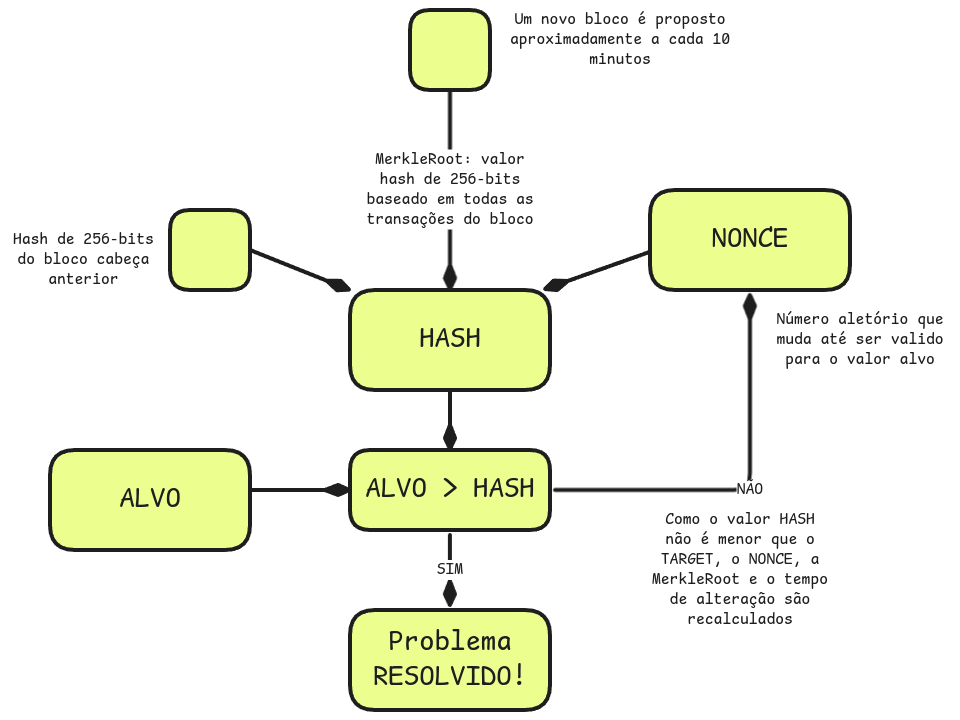
\includegraphics[width=0.8\textwidth]{figures/bitcoinmining.png}
		\caption{Mineração no Bitcoin.\ \textit{Autoria própria}.}
		\label{fig:bitcoinmining}
	\end{figure}

\end{frame}

\begin{frame}{Desafios do Proof of Work (PoW)}

	\begin{itemize}
		\item \textbf{Risco de 51\%:} Se uma entidade controlar 51\% ou mais da
		      rede, poderá manipular a blockchain, aprovando transações fraudulentas e
		      revertendo transações legítimas.
		\item \textbf{Processo demorado:} Mineradores testam muitos valores de
		      \textit{nonce} até encontrar a solução do problema criptográfico, tornando
		      o processo lento.
		\item \textbf{Alto consumo de recursos:} A mineração de Bitcoin exige grande
		      poder computacional, consumindo 55,27 TWh em 2019 (0,24\% do total mundial),
		      um aumento expressivo em relação a 2017 (5,027 TWh, 0,02\%). Esse
		      crescimento reflete a intensidade energética da mineração, que utiliza
		      hardware especializado e opera continuamente, gerando preocupações
		      ambientais e econômicas.~\cite{kufeoglu2019energy}
		\item \textbf{Transações não instantâneas:} O tempo de confirmação varia de
		      10 a 60 minutos, pois as transações precisam ser mineradas e adicionadas à
		      blockchain antes de serem finalizadas.
	\end{itemize}

\end{frame}
